%%%%%%%%%%%%%%%%%%%%%%%%%%%%%%%%%%%%%%%%%%%%%%%%%%%%%%%%%%%%%%%
% rjw 11/25/18 Make subsection of the Validation section 
% 1/9/19 Move back to just after the Introduction.
%
\subsection{Simulation}
\label{sec:fdsp-pd-simphys}
%\metainfo{(Length: \dword{tdr}=50 pages, TP=20 pages)}
%\metainfo{\color{blue} Content: Conveners}
% Provided by Alex H. 15mar18
%\metainfo{Content: Himmel}

%Content update by AH nov 2018
%edits by rjw nov 2018

The broad performance specifications for the \dword{pds} are determined by a series of physics deliverables addressing the major physics goals of DUNE: nucleon decay searches, supernova burst neutrinos, and beam neutrinos. Detailed subdetector specifications, such as light yield of the light collectors, are determined using a full simulation, reconstruction, and analysis chain developed for the \larsoft framework. 
%\fixme{I'm confused: the goals determine the needed sim/reco/analysis work which determines the requirements, which in turn determine the deliverables? Or the goals determine the deliverables, which determine the sim/reco/analysis work, which determines the requirements? Anne}
%The major physics goals of DUNE -- nucleon decay searches, \dword{snb} neutrinos, and beam neutrinos -- determine a series of physics deliverables.  The \dword{pds} requirements flow from the physics needs, determined using a full simulation, reconstruction, and analysis chain developed for the \larsoft framework. 

%The goal is to evaluate the performance in physics deliverables for each of the photon collector designs under consideration. The metrics evaluated will include efficiency for determining the time of the event ($t_0$), timing resolution, and calorimetric energy resolution for three physics samples: \dword{snb} neutrinos, nucleon decay events, %\footnote{The most relevant sample is actually the \emph{background} to nucleon decay events. However, efficiently simulating background that can mimic nucleon decays is challenging since they can be quite rare topologies, so it is easier to simulate the nucleon decay signal which should be representative of the background.}, 
%and beam neutrinos. However, the development of analysis tools to take advantage of this full simulation chain is fairly recent, so this proposal will only include one test case: $t_0$-finding efficiency for \dword{snb} neutrinos versus the effective area of the photon collectors (see Section~\ref{sssec:photoncollectors}).


\subsubsection{Simulation and Reconstruction Steps} 

The first step in the simulation specific to the \dword{pds} is the simulation of the production of light and its transport within the volume to the \dwords{pd}. Argon is a strong scintillator, producing \SI{24000}{$\gamma$s/MeV} at our nominal drift field. Even accounting for the efficiency of the \dwords{pd}, it is prohibitive to simulate every optical photon with \dword{geant4} in every event. So, prior to the full event simulation, the detector volume is voxelized and many photons are produced in each voxel. The fraction of photons from each voxel reaching each photosensor is called the visibility, and these visibilities are recorded in a 4-dimensional library (akin to the photon maps used in the \dword{dpmod} simulation described in \voltitledp~Chapter~5).
%\fixme{This reference to DP chapter 5 is hardwired - check this is the correct chapter number.}
This library includes Rayleigh scattering length ($\lambda=$ \SI{60}{cm}\cite{Grace:2015yta}), absorption length ($\lambda=$ \SI{20}{m}), and the measured collection efficiency versus position of the double-shift light-guide bars. When a particle is simulated, at each step it produces charge and light. The light produced is distributed onto the various \dwords{pd} using the photon library as a look-up table and the 30\% early (\SI{6}{ns}) plus 70\% late (\SI{1.5}{$\mu$s}) scintillation time constants are applied. Transport time of the light through the \lar is not currently simulated, but is under development.

The second step is the simulation of the sensor and electronics response. For the studies shown here, the SensL \dword{sipm} and \dword{sipm} signal processor (\dword{ssp}) readout electronics used for \dword{pd} development and in \dword{pdsp} is assumed (see Section~\ref{sec:fdsp-pd-pde}). However, a range of \dword{s/n} and dark rates are considered in order to set requirements on the needed performance of the electronics.
%Waveforms are produced on each channel by adding an \dword{sipm} single-\phel response shape for each true photon. In addition, other characteristics of the \dword{sipm} are included such as dark noise, and crosstalk, based on data from device measurements. 
%) From Alex 4/17/18 - We do include afterpulsing as well, at rates based on the sensl sipm's tested in Hawaii. You can just add it to the list of things included in the electronics simulation. 
Crosstalk (where a second cell avalanches when a neighbor is struck by a photon generated internal to the silicon) is introduced by adding a second \phel \num{16.5}\% of the time when an initial \phel is added to the waveform. Additional uncorrelated random noise is added to the waveform with an RMS of %\SI{2.6}{ADC} (or approximately 
\SI{0.1}{\phel{}}. The response of the \dword{ssp} self-triggering algorithm, based on a leading-edge discriminator, is then simulated to determine if and when a \SI{7.8}{$\mu$s} waveform will be read out, or in the case of the simulation, %it will be 
stored and passed on for later processing.

The third step is reconstruction, which proceeds in three stages. The first is a ``hit finding'' algorithm that searches for peaks on individual waveforms channel-by-channel, identifying the time (based on the time of the first peak) and the total amount of light collected (based on the integral until the hit goes back below threshold). The second step is a ``flash finding'' algorithm that searches for coincident hits across multiple channels. All the coincident light is collected into a single object that has an associated time (the earliest hit), an amount of light (summed from all the hits), and a position on the plane of the \dwords{apa} ($y$-$z$) that is a weighted average of the positions of the photon collectors with hits in the flash. %\footnote{Currently, the flash reconstruction does not consider the positions of the hits, only their times. This will need to be updated in the future when we simulate the full-sized \dword{spmod} but for now we are working in a small test geometry that acts as a crude simulation of this kind of constraint.}. 
The final step is to ``match'' the flash to the original event by taking the largest flash within the allowed drift time that is within \SI{240}{cm} in the $y$-$z$ plane. Since the TPC reconstruction is still in active development, especially for low-energy events, we match to the true event %\dword{mc} 
vertex of the event in the analyses presented here. This is a reasonable approximation since the position resolution of the TPC will be significantly better than that of the \dword{pds}. 

These tools (or subsets of them) are then used to evaluate how the performance of the \dword{pds} affects the following set of physics deliverables.

\subsubsection{Nucleon Decay}

Nucleon decays are rare events, so excluding backgrounds is of the utmost importance. Since some backgrounds can be generated by cosmic rays passing outside the active detector area, setting a fiducial volume to exclude such events is critically important.

\textit{Fiducialization with \tzero}
The physics deliverable: the \dwords{pd} must be able to determine \tzero with approximately \SI{1}{\micro s} resolution (SP-FD-4: time resolution) for events with visible energy greater than \SI{200}{MeV} throughout the active volume, and do so with $>99\%$ efficiency (SP-PDS-1: light yield uniformity). This energy regime is relevant for nucleon decay and atmospheric neutrinos. The time measurement is needed for event localization for optimal energy resolution and rejection of entering backgrounds. 
This resolution is required for comparable spatial resolution to the TPC along the drift direction.

\begin{dunetable}[PDS efficiency for nucleon decay events.]
{ccc}
{tab:pds-ndk}
{Efficiency for tagging nucleon decay events at the \dword{cpa} (\SI{3.6}{m} from the \dwords{pd} ) with the \dword{pds}  for a range of ``effective area'' (efficiency times active area) per module and the equivalent light yield per MeV at the \dword{cpa}.}
Effective Area (cm$^{2}$) & Light Yield at \dword{cpa} (PE/MeV) & Efficiency at the \dword{cpa} \\ \toprowrule
4.1   & 0.09 & $93.8 \pm 0.4$ \\ \colhline
12.8  & 0.28 & $97.7 \pm 0.4$ \\ \colhline
15.0  & 0.33 & $98.4 \pm 0.2$ \\ \colhline
23.0  & 0.50 & $98.9 \pm 0.2$ \\ 
\end{dunetable}


The physics here feeds down to a requirement on the light yield in the dimmest regions of the detector (SP-PDS-1: light yield uniformity), determined by measuring how often the correct flash was not assigned to nucleon decay 
events\footnote{The most relevant sample is actually the \textit{background} to nucleon decay events. However, efficiently simulating background that can mimic nucleon decays is challenging since they can be quite rare topologies. It is therefore easier to simulate the nucleon decay signal that should be representative of the background.} 
verses distance from the \dword{apa} and versus the efficiency of the \dwords{pd} using the full simulation and reconstruction described in the previous section. The results of the simulation studies are shown in Table~\ref{tab:pds-ndk}. A light collector design that achieves \SI{23}{cm^2} effective area equivalent to a light yield of \SI{0.5}{PE/MeV} at the CPA) meets the requirement of 99\% efficiency at the \dword{cpa}.


\subsubsection{Supernova Neutrinos}

Supernova bursts are also rare events, though here the event is made up of many interactions instead of a single interaction. For distant supernovae (at the far side of the Milky Way or in the Large Magellanic Cloud), the top priority is to ensure that the detector can identify a burst when it happens and trigger the detector readout. For nearby supernovae, triggering will not be a challenge, and instead the goal is to record as much information as possible about the burst.

\textit{Burst Triggering}

The physics deliverable: the \dword{pds} must be able to trigger on \dwords{snb} in our galaxy and the Large Magellanic Cloud with efficiency similar to the TPC, with a false positive rate of less than one per month. This deliverable is most important for distant supernovae where the most important requirement is that we trigger and record the data. The \dword{pds}-based trigger should have similar performance to the TPC trigger so they can provide redundancy against one another or be combined to increase efficiency or lower the background rate. The once-per-month false positive rate is determined by limits from the \dword{daq} and data handling.

The \dword{pds} trigger performance was studied for a plausible but challenging signal: a supernova burst in the Large Magellanic Cloud, which we conservatively assumed would produce only 10 signal events in the far detector. The trigger efficiency was studied with variations in light yield (e.g. effective area), dark rate, and signal-to-noise ratio, keeping the requirement from the DAQ that the fake rate be held to less than one per month. The burst trigger efficiency, found to be approximately $80\%$, is relatively insensitive to all these parameters for effective areas $>$\SI{15}{cm^2} (average light yield $>$\SI{7}{PE/MeV}), dark rate $<$\SI{1}{kHz}, and signal-to-noise $>3$. The uncorrelated noise from dark rate and low signal-to-noise was easily excluded from trigger primitives by the clustering scheme, and the increased effective area makes both backgrounds and signal brighter together so performance stays basically constant. Thus this physics deliverable, while important, does not constrain any detector requirements.



\textit{TPC Energy Measurement and Time Resolution with \tzero}

The physics deliverable: the \dwords{pd} must be able to provide \tzero determination with approximately \SI{1}{\micro s} resolution (SP-FD-4: time resolution) for at least 60\% of the neutrinos in a typical \dword{snb} energy spectrum. The \tzero's are used in concert with the TPC-reconstructed event in two ways: to correct for the attenuation of the charge signal as a function of how far the charge drifts through the TPC and to provide more precise absolute event times for resolving short time features in the \dword{snb} neutrino event rate. This deliverable is important primarily for nearby supernovae where the number of events is large enough that time and energy resolution will be the limiting factors in extracting physics. 

\begin{dunefigure}[Supernova neutrino energy resolution from the TPC for different PD performance assumptions.]
{fig:pds-snb-driftcor}
{The energy resolution for supernova neutrino events when reconstructed by the TPC and drift corrected with varying assumptions on the performance of the \dwords{pd}, parameterized by effective area, $A_{eff}$. The options considered range from drift correction for no events (black), to 60\% of events (blue), to 100\% of events (red).
}
  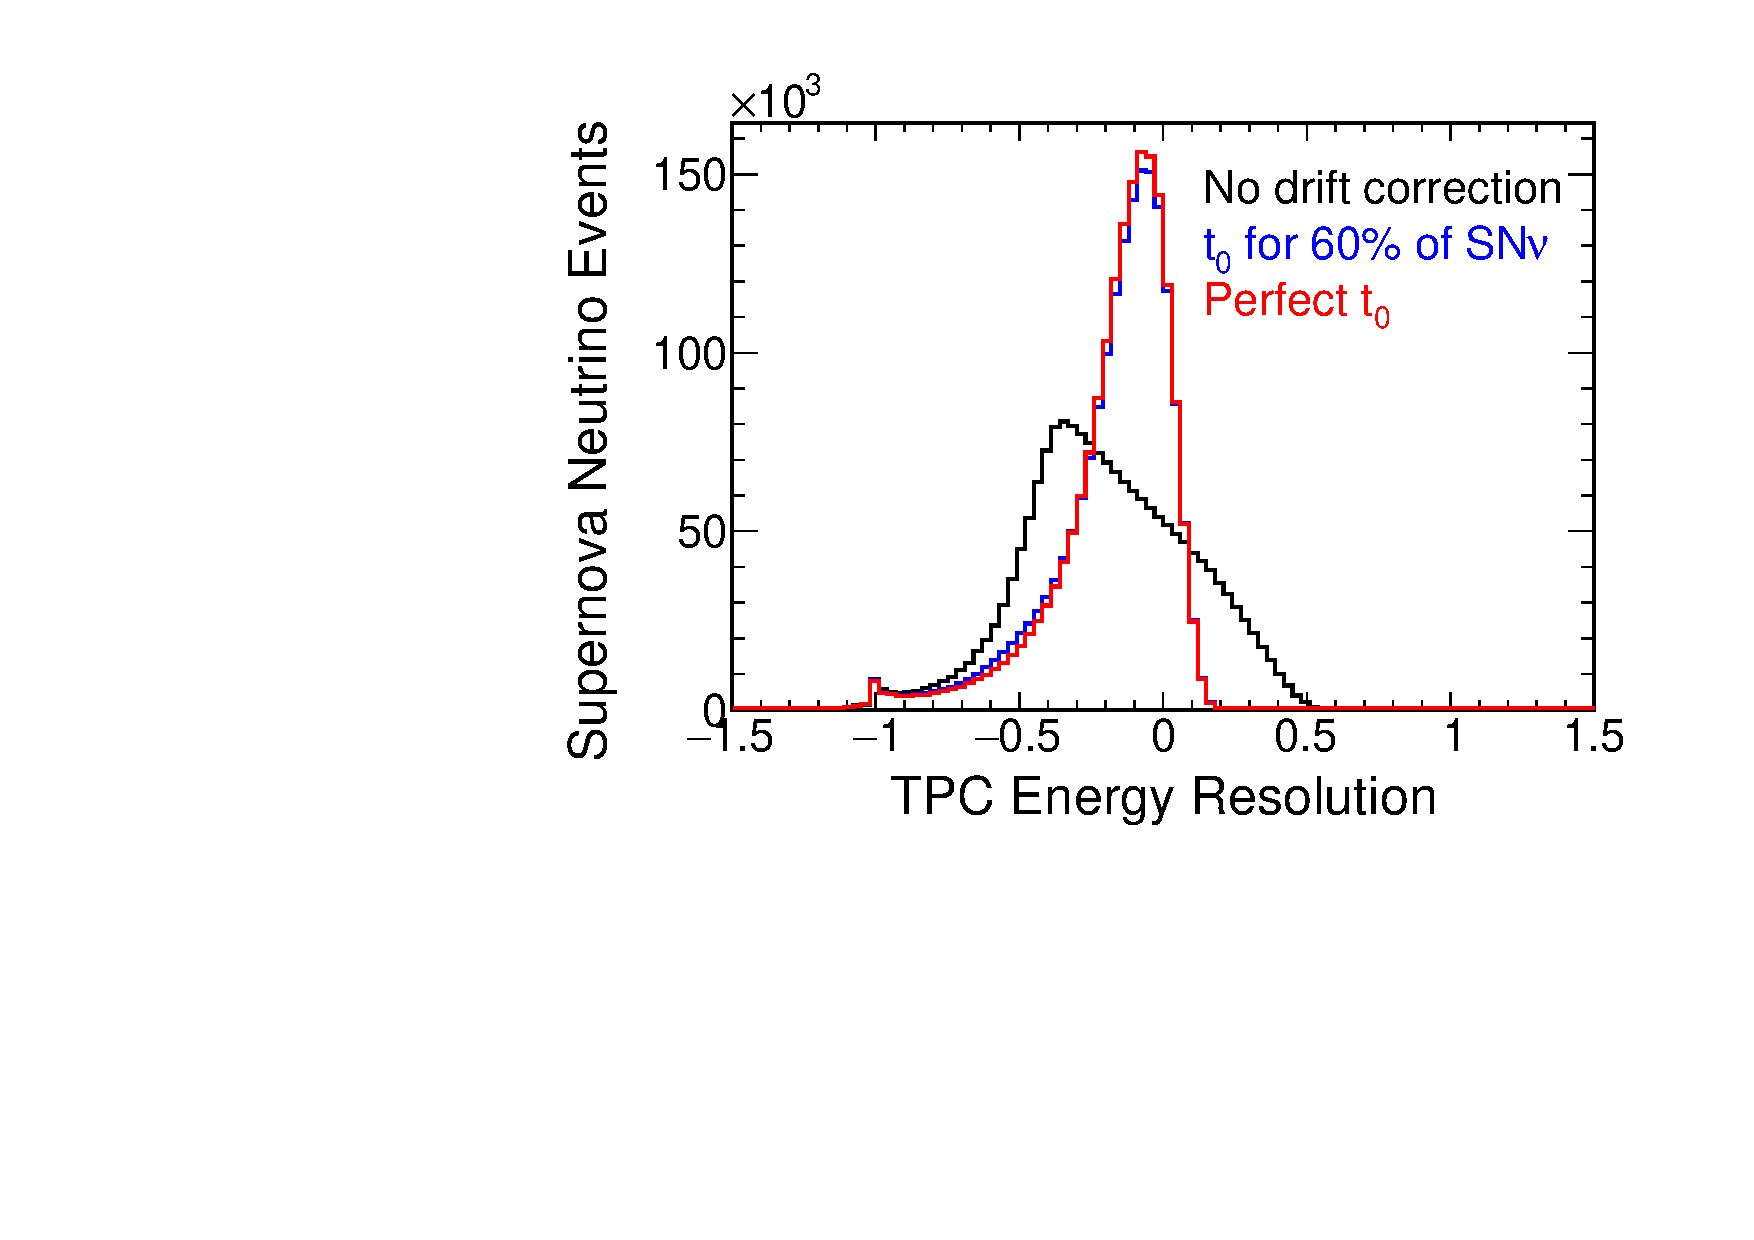
\includegraphics[width=0.6\textwidth]{graphics/pds-snb-drift-corr}
 \end{dunefigure}

The 60\% \tzero tagging requirement comes from two studies of a typical \dword{snb} neutrino spectrum under varying \dword{pd} performance assumptions: the resolution of the energy reconstructed with the TPC and drift-corrected using the time from the \dwords{pd}, and the observability of the in-fall `notch' in the \dword{snb} event time distribution. Both studies show significant improvement when going from no \dwords{pd} to a system with an effective area of \SI{4.05}{cm^2} (equivalent to \SI{0.5}{PE/MeV} for 60\% of the detector volume), but only marginal improvements past that point. The light yield required here is sufficiently low that this deliverable does not set any detector requirements.


\textit{Calorimetric Energy}

Physics deliverable: the \dword{pds} should be able to provide a calorimetric energy measurement for low-energy events, like \dwords{snb}, complementary to the TPC energy measurement. 
Improving the energy resolution, up to the fundamental limits imposed by invisible particles in the interaction, will enable us to extract the maximum physics from a \dword{snb}, and with the goal to achieve energy resolution comparable to the TPC, we can take full advantage of the anti-correlation between the emission of light and charge signals imposed by the conservation of energy.


\begin{dunefigure}[Supernova neutrino energy resolution from the PDS for different PD performance assumptions.]
{fig:pds-snb-calo}
{The energy resolution (determined from the distribution widths of the fraction of difference between reconstructed and true  to true neutrino energy for simulated events) for supernova neutrino events when reconstructed directly through \dword{pds} calorimetry for a range of detector performance assumptions, represented by different colors. The red line on the left plot labeled {\it Physics} 
shows the energy smearing inherent to the neutrino interactions and thus serves as a theoretical minimum resolution. The behavior vs. true and reco energy looks different because some higher energy neutrinos lose otherwise visible energy into neutrons, causing the poorly resolved higher true energy events to all feed down to lower reconstructed energies. Even with these differences, both plots show that the performance improves significantly up through effective area of \SI{30}{cm^{2}}, but improvements past that point become quite small. By comparison, the black line on the left plot shows the TPC energy resolution (with drift correction from the \dword{pds}) is approximately $25\%$.
}
  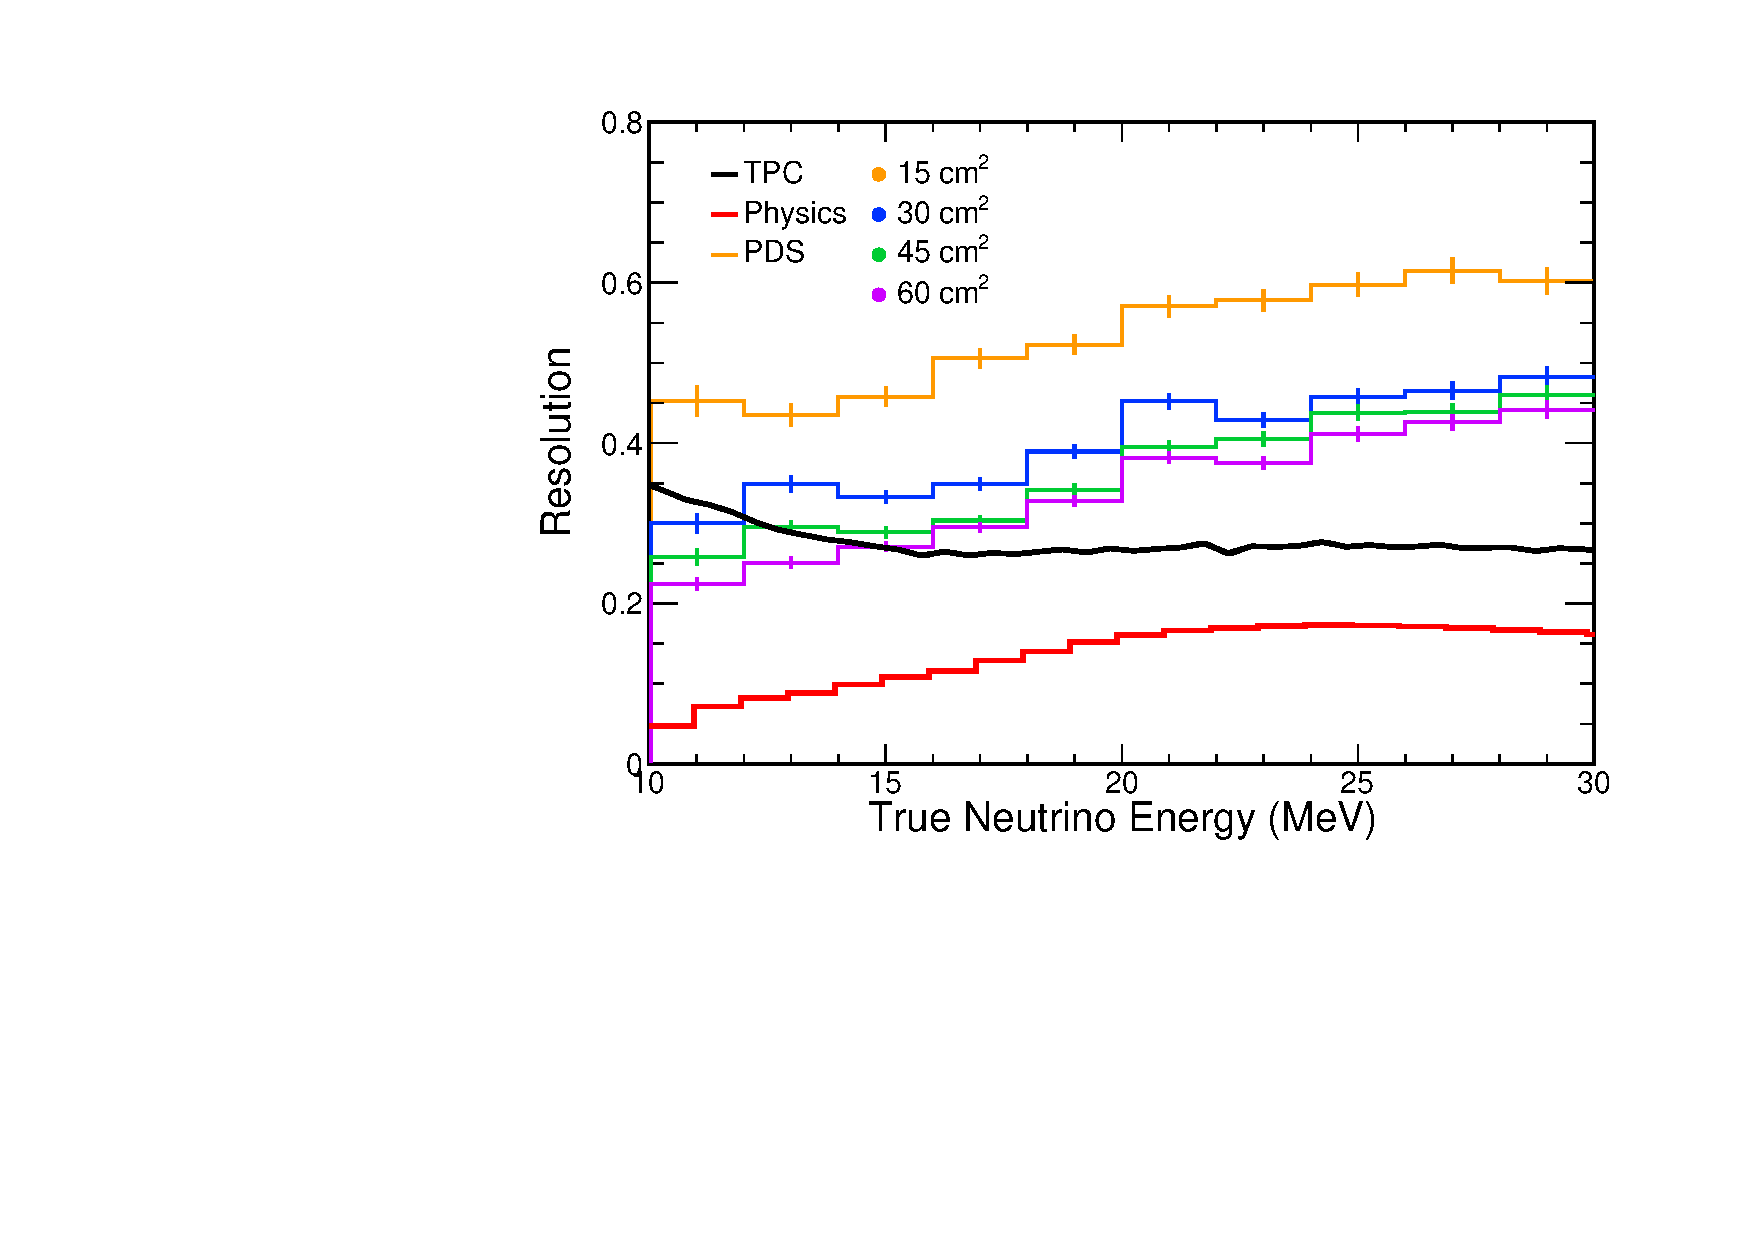
\includegraphics[width=0.48\columnwidth]{graphics/pds-snb-res-vs-true.pdf}
  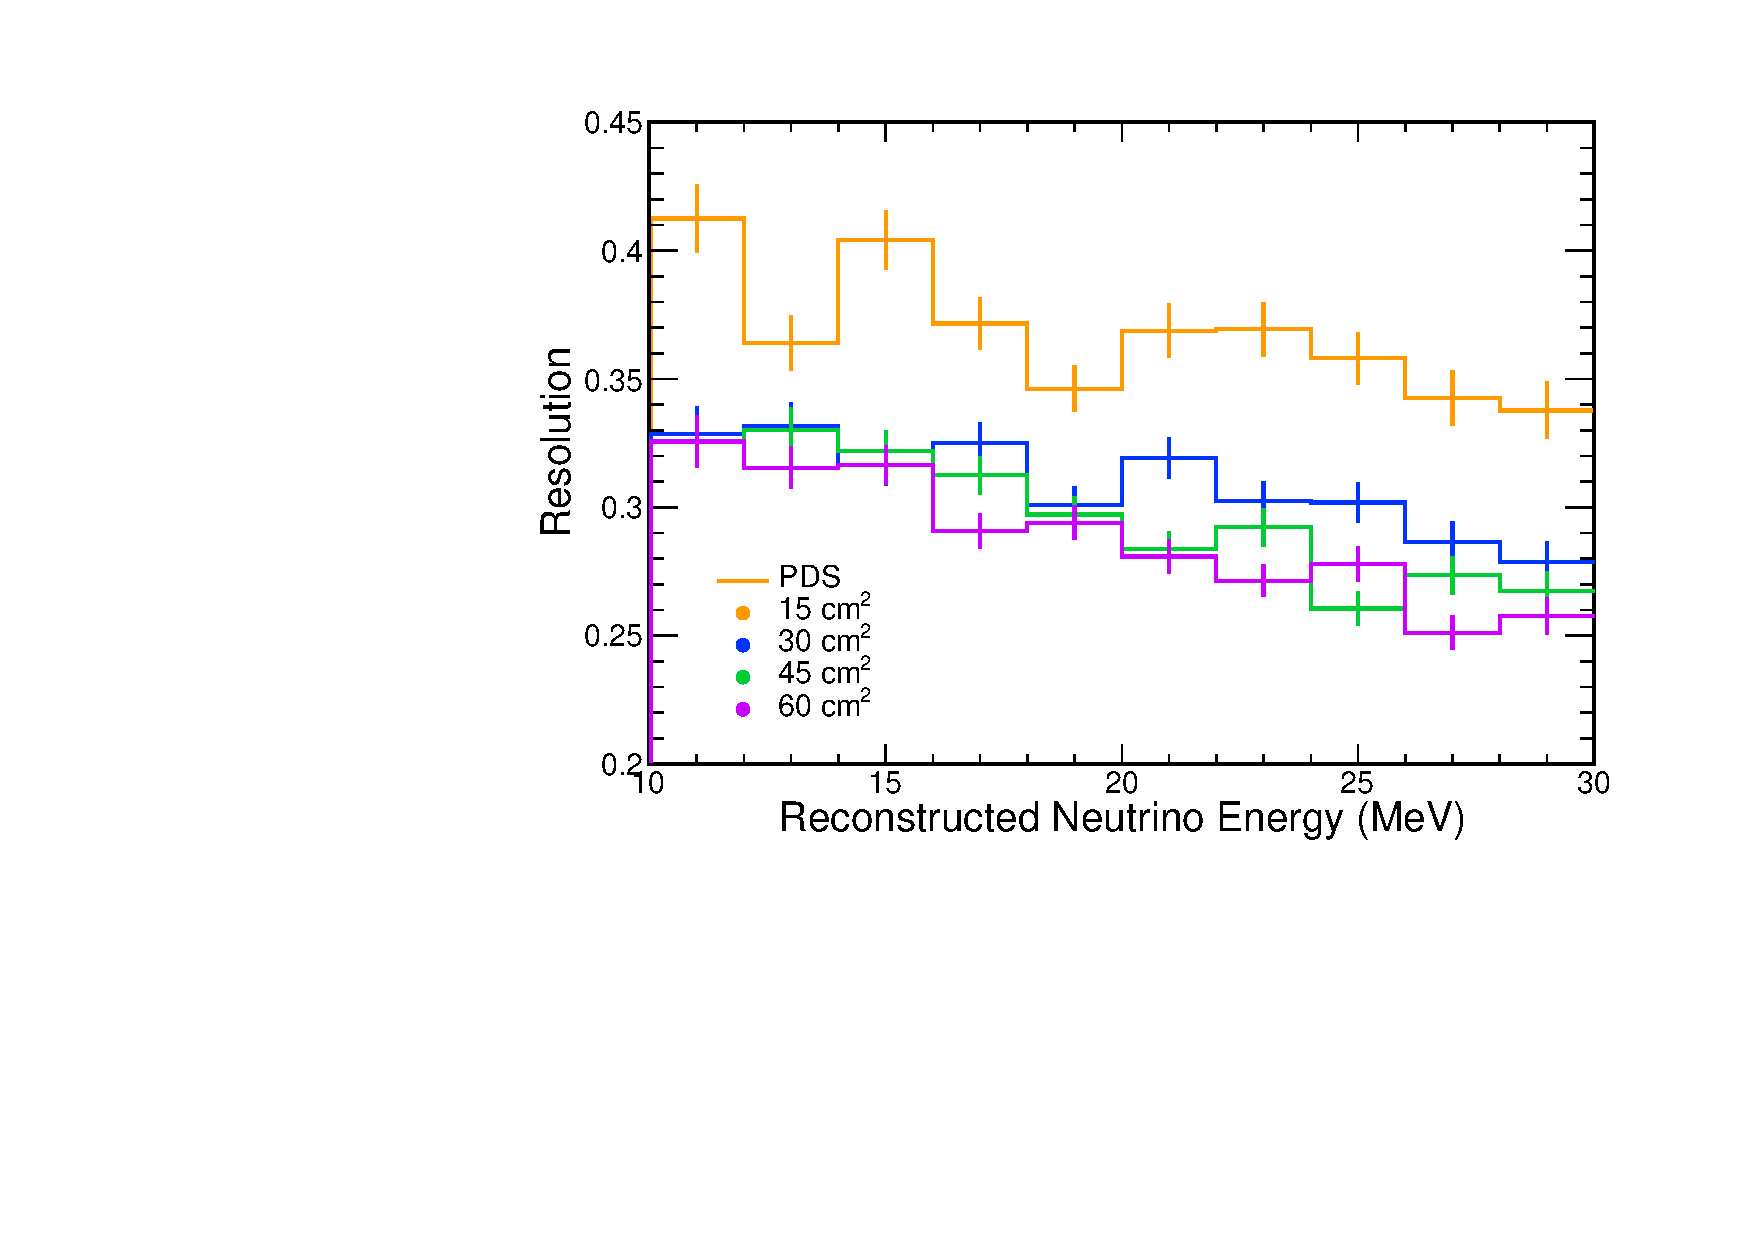
\includegraphics[width=0.48\columnwidth]{graphics/pds-snb-res-vs-reco.pdf}
 \end{dunefigure}

The calorimetric energy performance was studied for supernova burst neutrino events simulated in the far detector for a range of different detector performance assumptions. The energy reconstruction was simple, correcting the total observed amount of photons for the average number of photons expected per MeV as a function of position along the drift direction. Events were required to be well away from the side walls to avoid any possible edge effects. The energy resolution vs. true and reconstructed energy is shown in Fig.~\ref{fig:pds-snb-calo}. The behavior looks notably different between the two plots because there is an asymmetric bias which begins at higher energies due to loss of otherwise visible energy into neutrons. However, both support the same conclusion: there is a significant benefit to achieving a photon detector with effective area of \SI{30}{cm^2} (average \SI{13}{PE/MeV}), but past that point improvements become relatively small. This physics deliverable thus sets a requirement, FD-SP-3: light yield, of \SI{13}{PE/MeV} averaged over the active volume.

\subsubsection{Beam Neutrinos}

The \dword{pds} is not needed for fiducializing beam neutrino events since the pulsed beam will provide sufficient precision to place the interactions in space. However, the \dwords{pd} can potentially contribute to the energy measurement and the better timing resolution can help identify Michel electrons from muon and pion decay.


\textit{\it Calorimetric Energy}

Physics deliverable: the \dword{pds} should be able to provide a calorimetric energy measurement for high-energy events, like neutrinos from the LBNF beam, complementary to the TPC energy measurement.
Neutrino energy is an observable critical to the success of the oscillation physics program, and a second independent measurement can provide a cross-check that reduces systematic uncertainties or directly improves resolution for some types of events. In order to provide a meaningful cross-check, the resolution and uncertainty of the \dword{pds} measurement must be comparable to the calorimetric resolution of the TPC. The limit on this measurement will likely come from how well the efficiency of the detector and the optical properties of the argon can be determined (both must be known to approximately 5\% to have a comparable measurement of electron shower energy), which define a program of measurements between now and the operation of the detector rather than requirements on the system itself. The requirement that does flow down from this is that the dynamic range of the system be sufficient to allow for accurate measurement of the amount of light reaching the \dword{pds}. 

Some amount of saturation is tolerable since it can be corrected for using the pulse shape or the neighboring unsaturated channels. However, if the saturation is too large, and too many channels are saturated, the corrections become difficult, so we require that no more than $20\%$ of beam neutrino events have saturating channels (SP-PDS-16: dynamic range), consistent with but looser than the \dword{tpc} requirement of $10\%$.

We studied the likelihood of channels saturating by simulating beam neutrino events in the far detector. The likelihood of saturation depends on the digitization frequency, the dynamic range, and the effective area (collection efficiency) of the detector design. Assuming the baseline electronics, a 12-bit and \SI{80}{MHz} digitizer, we find the likelihood of saturation vs. effective area shown in Table~\ref{tab:pds-dynamicrange}. 

\begin{dunetable}[Fraction of beam events with channels that saturate]
{ccc}
{tab:pds-dynamicrange}
{The fraction of beam events which have saturating \dword{pds} channels for different assumed detector effective areas.}
Effective Area (cm$^{2}$) & Fraction of Events with Saturation \\ \toprowrule
15   & $6\%$ \\ \colhline
30   & $13\%$ \\ \colhline
45   & $20\%$ \\ \colhline
60   & $24\%$ \\ 
\end{dunetable}


\textit{\it Michel Electron Tagging}

Physics deliverable: the \dword{pds} should be able to identify events with Michel electrons from muon and pion decays.
The identification of Michel electrons can improve background rejection for both beam neutrinos and nucleon decay searches. 
Some Michel electrons are difficult to identify with the TPC since they appear simultaneous within the time resolution of the TPC and collinear with their parent. However, because the \dword{pds} can observe the fine time structure of events in the detector, it can identify Michel electrons that appear separated in time from the main event. While DUNE-specific studies of Michel electron tagging have not been performed, the LArIAT experiment has demonstrated that Michel electrons can be identified and studied using photon signals.

%\fixme{Add LArIAT reference once it exists}

